\chapter{Illustrative Example of use of CIPRNGs in the Computer Science Security Field}
\label{State-of-the-art}

This chapter is devoted to a first application of CIPRNGs to see whether they still remains
good in concrete situations. The publication of \cite{bfg12b:ip} has formally given a description of this research.

\section{Introduction}

The confidentiality of information transmitted through the Internet requires an intensive use of pseudorandom number generators having strong security properties. For instance, these generators are used to produce encryption keys, to encrypt data with a one-time pad process, or to dissimulate information into cover media. In our previous chapters, we have shown how to use  discrete chaotic iterations to build pseudorandom number generators, by receiving two inputted possibly deficient generators, and mixing them to produce pseudorandom numbers with high statistical qualities. In this chapter, 
%we summarize these contributions and
 we propose simple basic applications of these generators for encryption and information hiding. For each application, first experimental evaluations are given, showing that an attacker using these statistics as detection tools cannot infer the presence of an hidden message into given cover documents.

%
%
%The extremely rapid development of the internet brings more and more attention to information security techniques, such as text encryption, e-Voting, digital rights management, etc~\cite{Gonzaleza2005}. Meanwhile chaos nowadays attracts lots of interests from researchers in the filds of mathematics, physics, and so on because of its connection with randomness and complexity~\cite{Behnia20113455, guyeux10}. Thus, various study works are focusing on the possibility to use chaos in random number generation for Internet security. Indeed, highly qualified random sequences generated from pseudorandom number generators (PRNGs), as an inseparable part of information hiding techniques, are urgently required.
%
%Since pseudorandom sequences are easy to be generated and processed, and due to their
%need in almost all cryptographic protocols and information hiding schemes, PRNGs (Pseudo Random Number Generators) are
%widely used for a secure Internet use.
%Among other things, they are part of the keys generation of any asymmetric cryptosystem,
%they produce keystreams in symmetric cryptosystems, they determine which bits will receive the
%secret message in information hiding, and so on.
%However, a lot of existing pseudorandom number generators (PRNGs) used in numerical simulations are eliminated for such applications, due to the requirements of speed, statistical quality, and security
%in that context.
\begin{figure*}
\centering
\subfigure[]{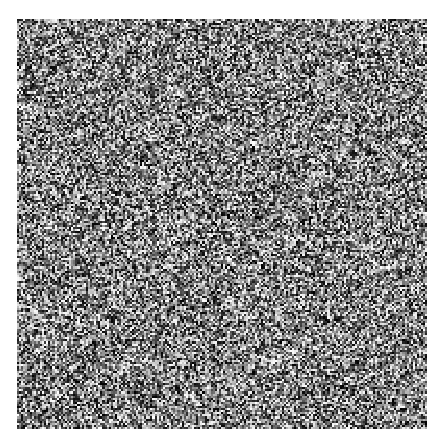
\includegraphics[scale = 0.55]{lena_crypt_old_ci.eps} %[Histogram of digitized laser]
}
\subfigure[]{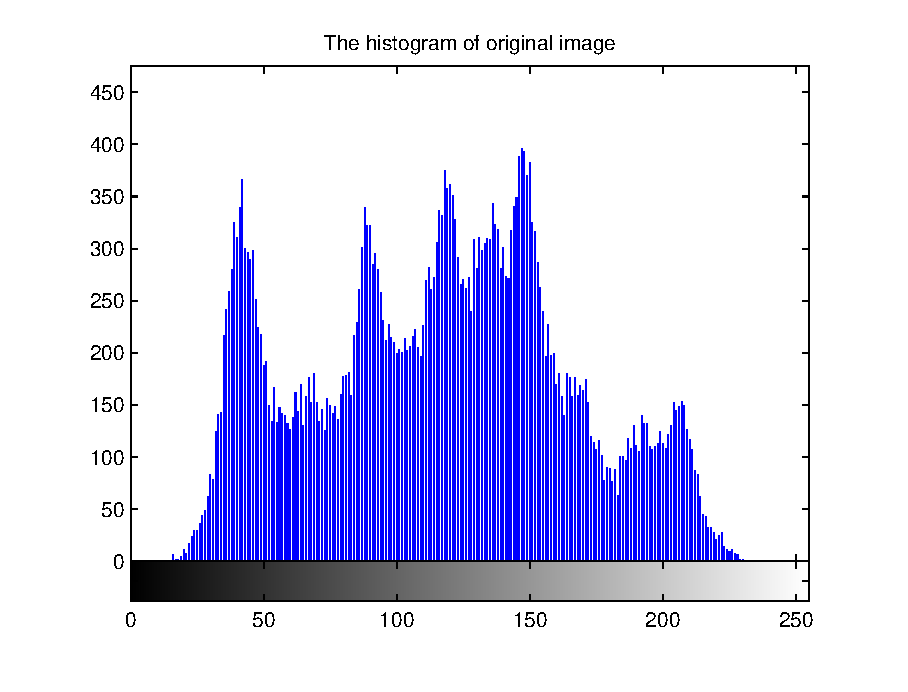
\includegraphics[scale = 0.35]{hist_old_ci.eps} %[Histogram of digitized laser]
}
\subfigure[]{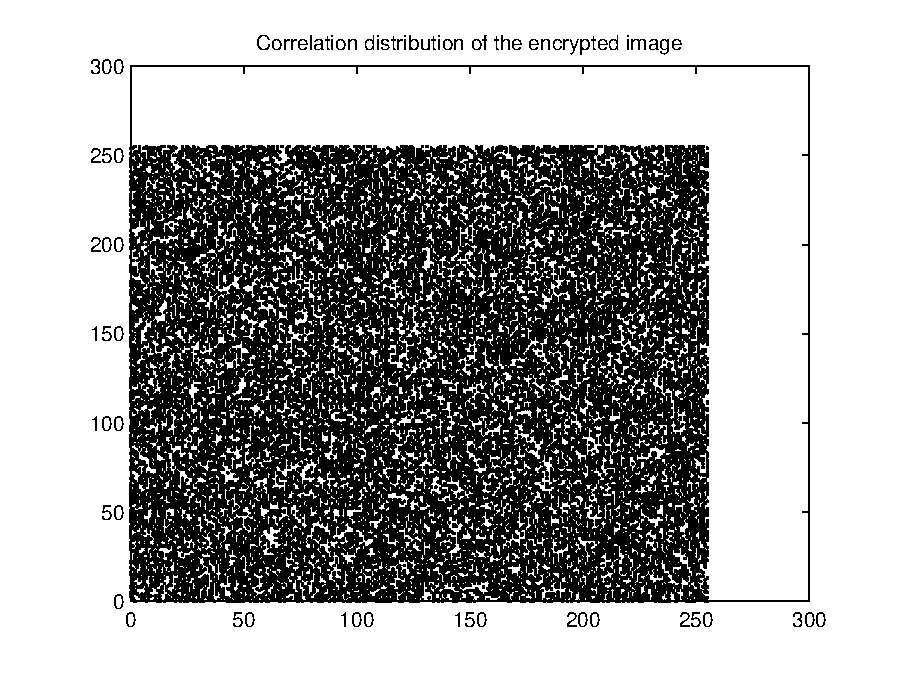
\includegraphics[scale = 0.35]{cd_old_ci.eps} %[Histogram of digitized laser]
}
\caption{(a) The encrypted Lena (one-time pad using Version 1 CI). (b) Histogram of Fig.(a). (c) Correlation distribution of two adjacent pixels in Fig.(a)}
\label{Old_CI}
\end{figure*}
%
\begin{figure*}
\centering
\subfigure[]{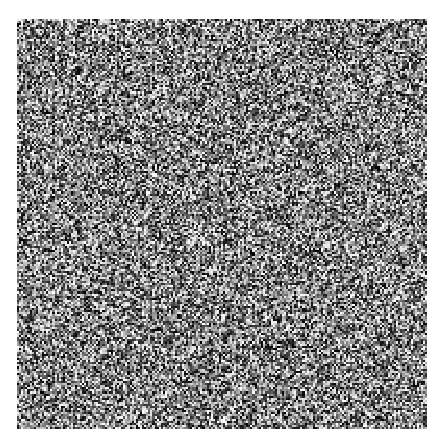
\includegraphics[scale = 0.55]{lena_crypt_new_ci.eps} %[Histogram of digitized laser]
}
\subfigure[]{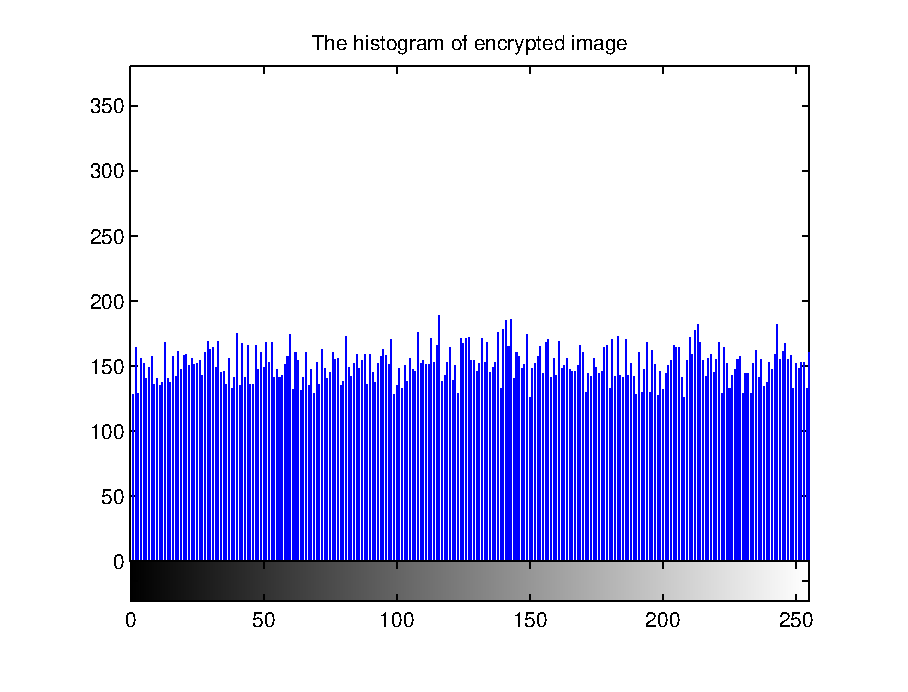
\includegraphics[scale = 0.35]{hist_new_ci.eps} %[Histogram of digitized laser]
}
\subfigure[]{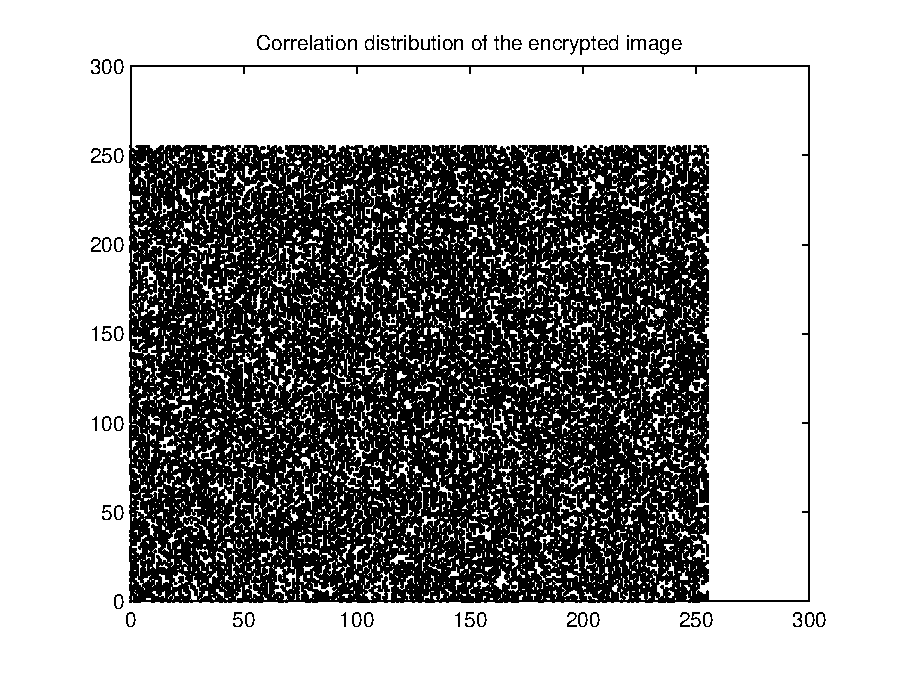
\includegraphics[scale = 0.35]{cd_new_ci.eps} %[Histogram of digitized laser]
}
\caption{(a) The encrypted Lena (one-time pad using Version 2 CI). (b) Histogram of Fig.(a). (c) Correlation distribution of two adjacent pixels in Fig.(a)}
\label{New_CI}
\end{figure*}
%Recent years, some researchers have investigated with success the use of chaotic dynamical systems to generate pseudorandom sequences~\cite{Hu20092286, DeMicco20083373}.
%Indeed, chaotic systems have many advantages as unpredictability or disorder-like, which are needed when producing complex sequences.
%They are extremely sensitive to the initial states too: a minute difference can cause a significant change in output.
%All these features fit well the requirements of PRNGs, thus explaining the proposal of such dynamics
%to secure exchanges.
%However, chaotic systems using real numbers on infinite bit representation, realized in finite computing precision, lead to short cycle length, non-ideal distribution, and other deflation of this kind.
%This is why chaotic systems on a infinite space of integers have been dig for these years, leading to the proposition to use chaotic iterations (CIs) techniques to reach the desired goals.
\begin{figure*}
\centering
\subfigure[]{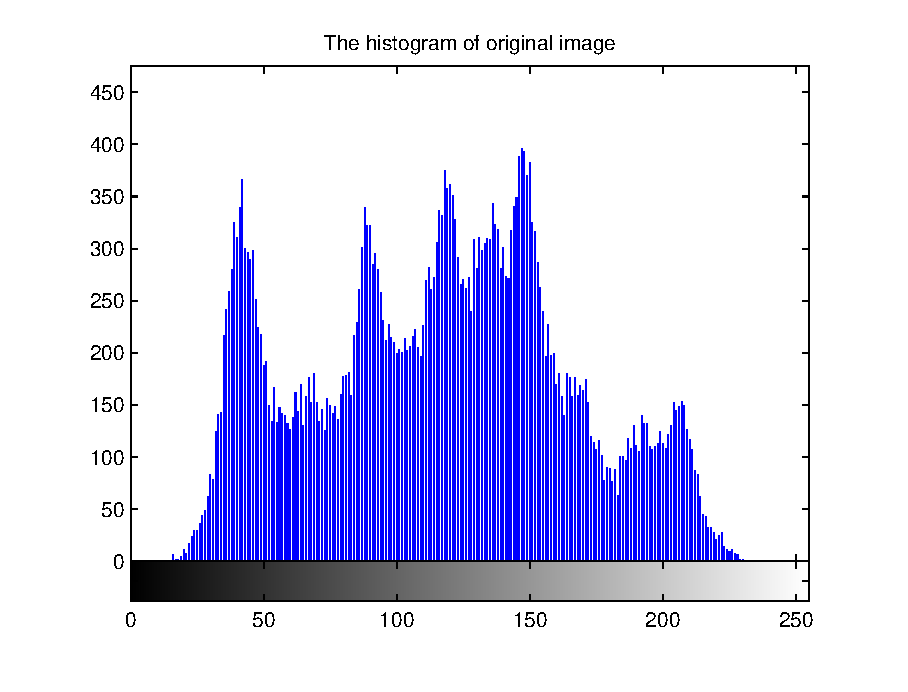
\includegraphics[scale = 0.29]{hist_old_ci.eps} %[Histogram of digitized laser]
}
\subfigure[]{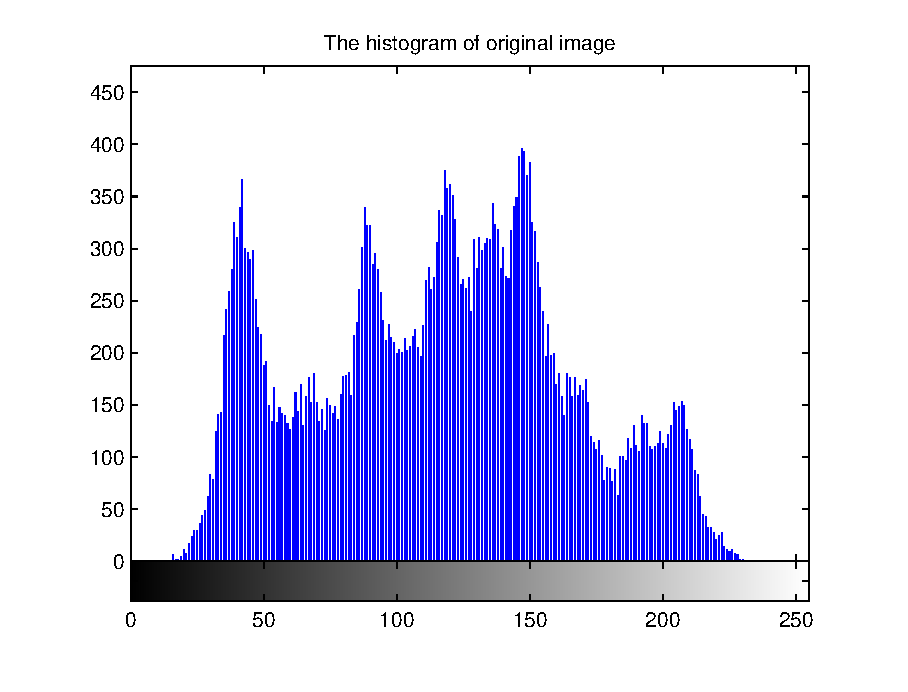
\includegraphics[scale = 0.29]{hist_old_ci_info.eps} %[Histogram of digitized laser]
}
\subfigure[]{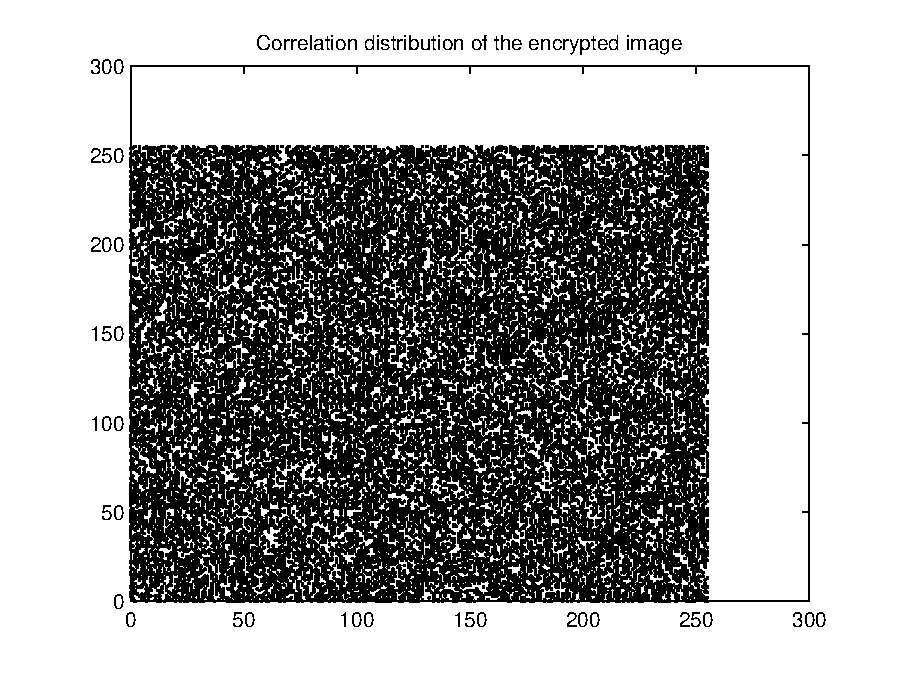
\includegraphics[scale = 0.29]{cd_old_ci.eps} %[Histogram of digitized laser]
}
\subfigure[]{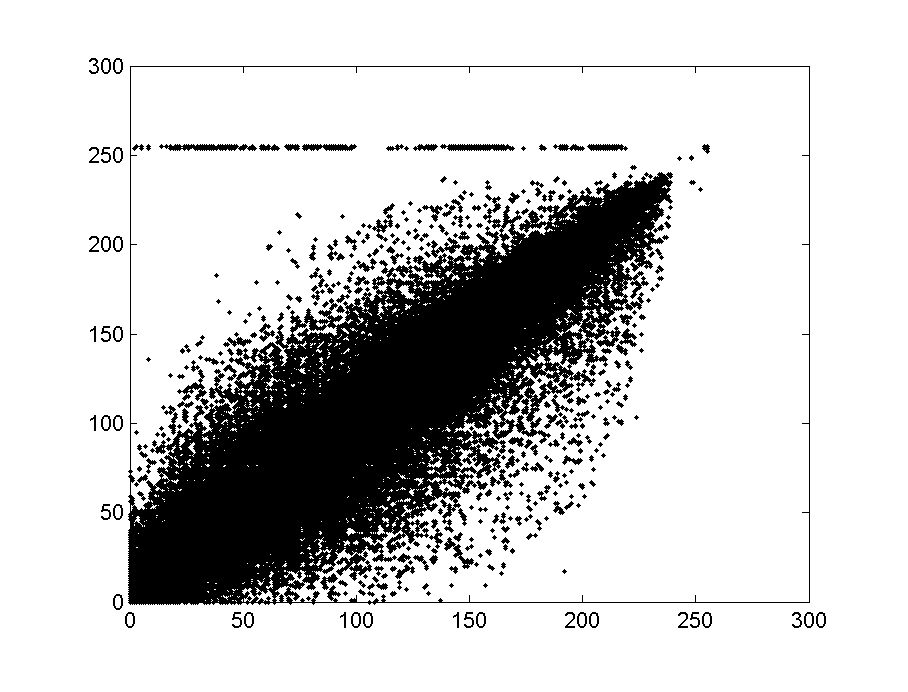
\includegraphics[scale = 0.29]{cd_old_ci_info.eps} %[Histogram of digitized laser]
}
\caption{ (a) Histogram of pixel values when LSBs are replaced by Version 1 CI. (b) Histogram of pixel values when LBSs are an hidden message xored with Version 1 CI. (c) Correlation distribution of two adjacent pixels in Fig.(a). (d) Correlation distribution of two adjacent pixels in Fig.(b).  }
\label{Old_CI_hiding}
\end{figure*}
\begin{figure*}
\centering
\subfigure[]{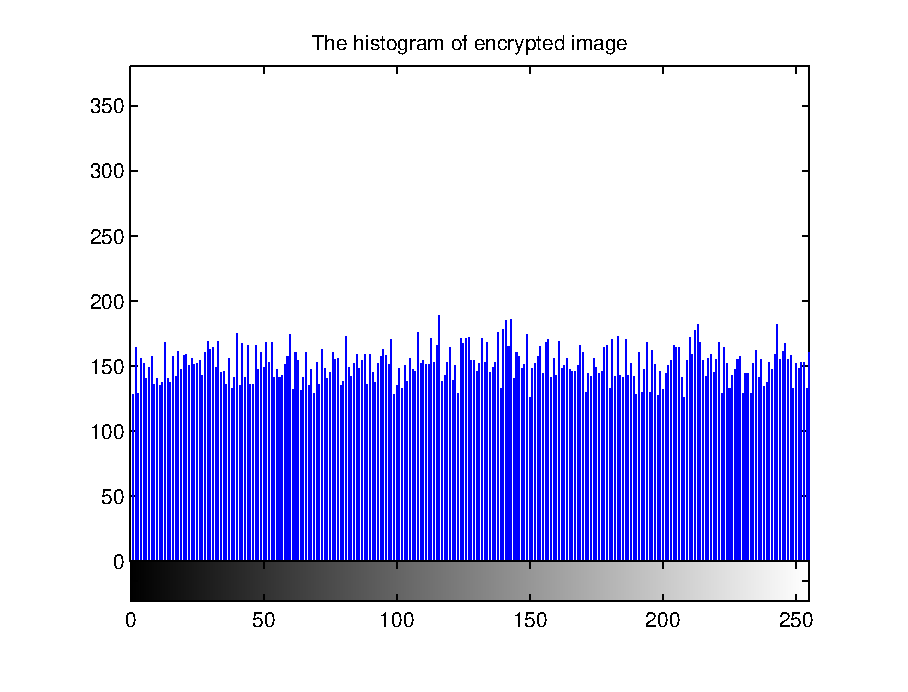
\includegraphics[scale = 0.29]{hist_new_ci.eps} %[Histogram of digitized laser]
}
\subfigure[]{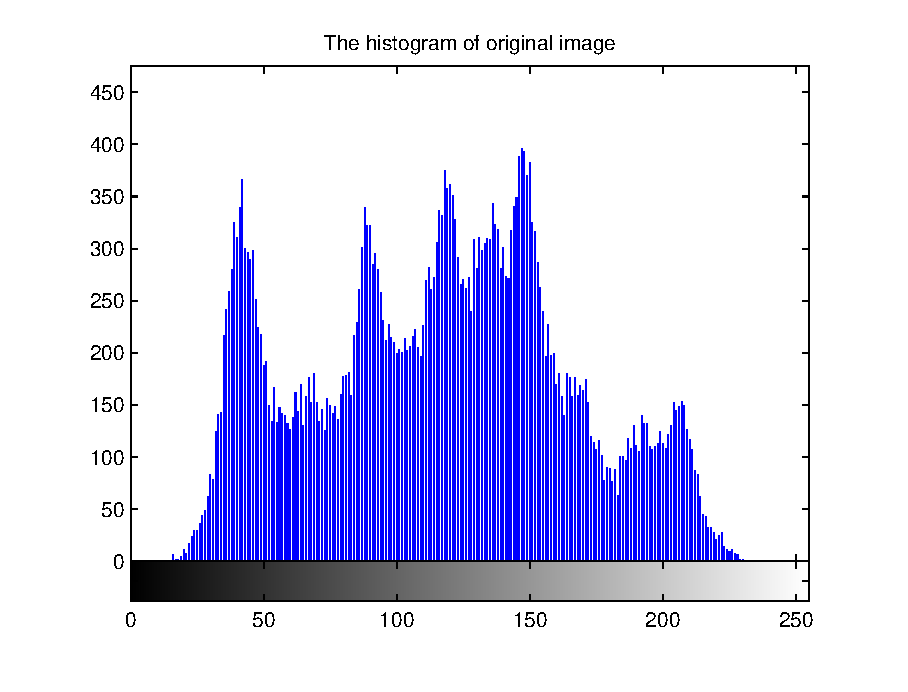
\includegraphics[scale = 0.29]{hist_new_ci_info.eps} %[Histogram of digitized laser]
}
\subfigure[]{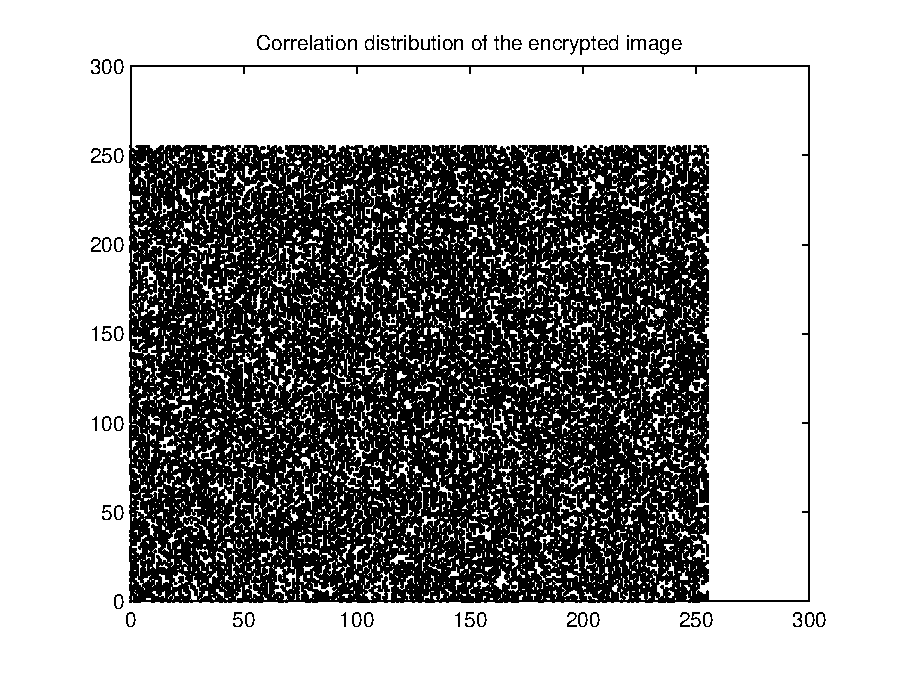
\includegraphics[scale = 0.29]{cd_new_ci.eps} %[Histogram of digitized laser]
}
\subfigure[]{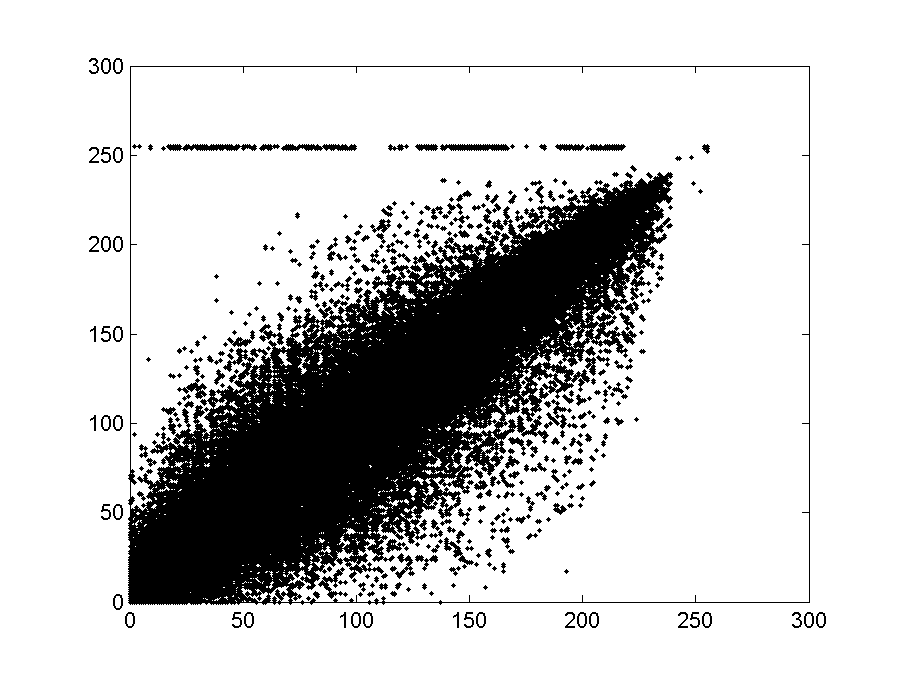
\includegraphics[scale = 0.29]{cd_new_ci_info.eps} %[Histogram of digitized laser]
}
\caption{ (a) Histogram of pixel values when LSBs are replaced by Version 2 CI. (b) Histogram of pixel values when LBSs are an hidden message xored with Version 2 CI. (c) Correlation distribution of two adjacent pixels in Fig.(a). (d) Correlation distribution of two adjacent pixels in Fig.(b).  }
\label{New_CI_hiding}
\end{figure*}
%The objective of this chapter is to make a state-of-the-art of chaotic iterations-based PRNGs, and to propose a possible use of them in the field of secrecy preservation through the Internet,
%by using information hiding techniques.
Random binary sequences will be generated by the three first CIPRNG methods using a XORshift generator.
The application of these pseudorandom bits for information hiding will be carried out systematically, and results will be discussed in order to verify that an attacker, who has only access to some elementary statistical tests,
cannot determine whether hidden information are embedded into cover documents or not.
Notice that the aim of this chapter is not to propose an up-to-date, finalized,
and secure data hiding scheme, but only to show the usability and effectiveness 
of our CIPRNGs.

\section{Application Evaluation}
\label{sec:application}

Let us firstly introduce our toy example in the information hiding security field. 

\subsection{The Proposed Information Hiding Method}

\begin{figure*}
\centering
\subfigure[]{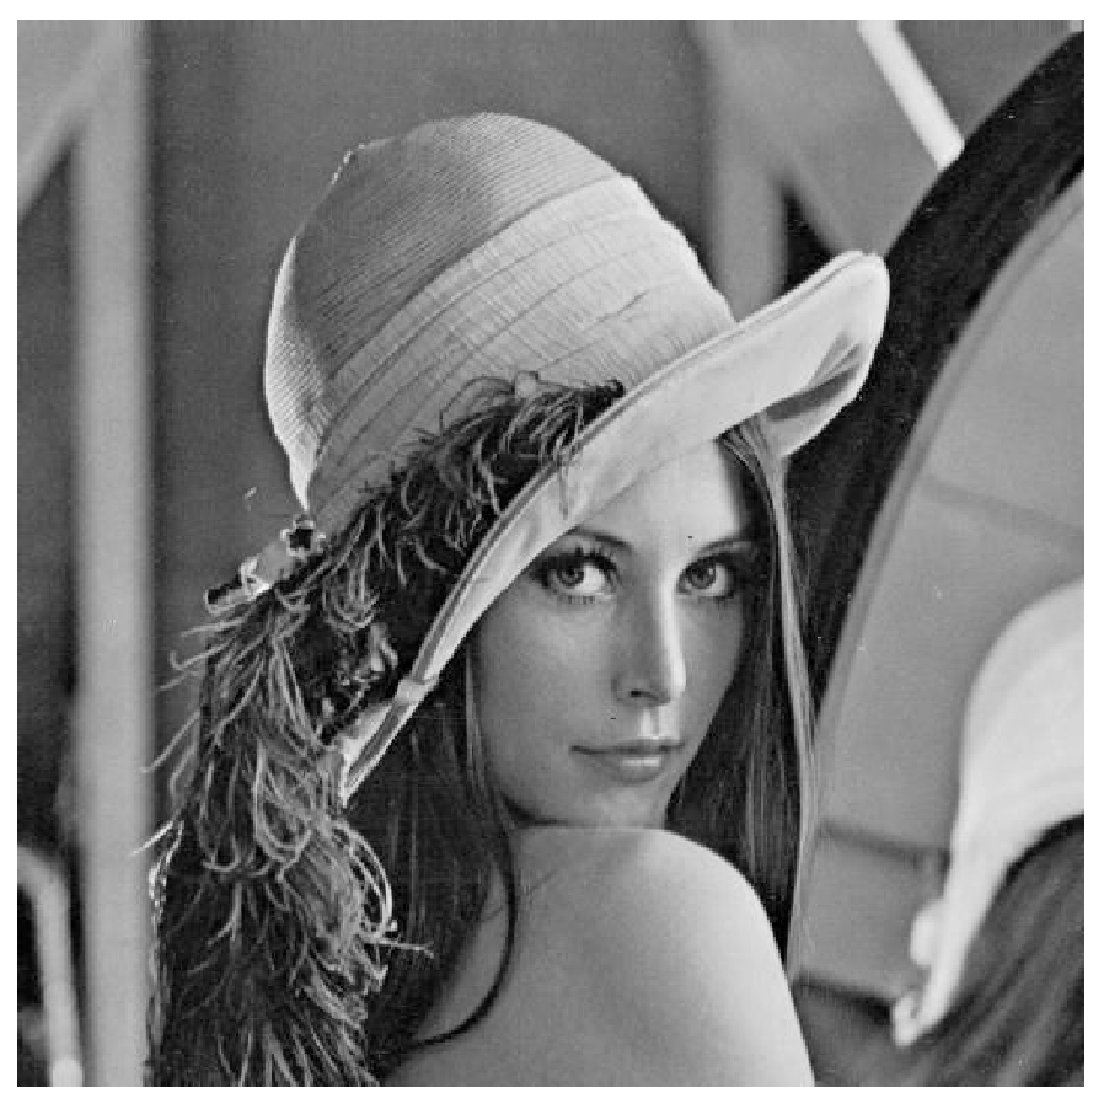
\includegraphics[scale = 0.15]{lena512.eps} %[Histogram of digitized laser]
}
\subfigure[]{
\includegraphics[scale = 0.35]{invader1.eps} %[Histogram of digitized laser]
}
\subfigure[]{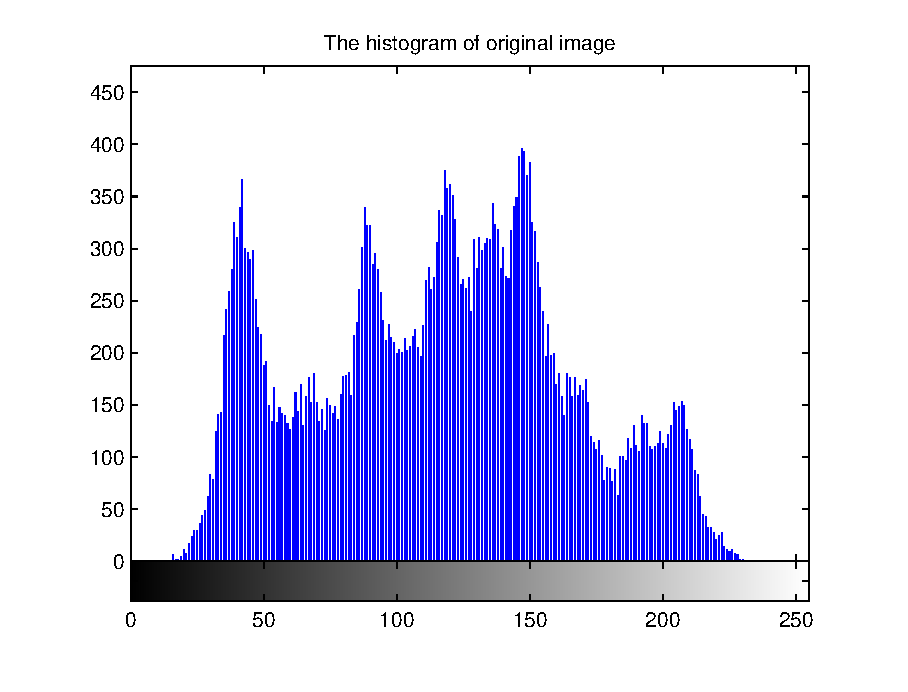
\includegraphics[scale = 0.35]{hist_lena.eps} %[Histogram of digitized laser]
}
\subfigure[]{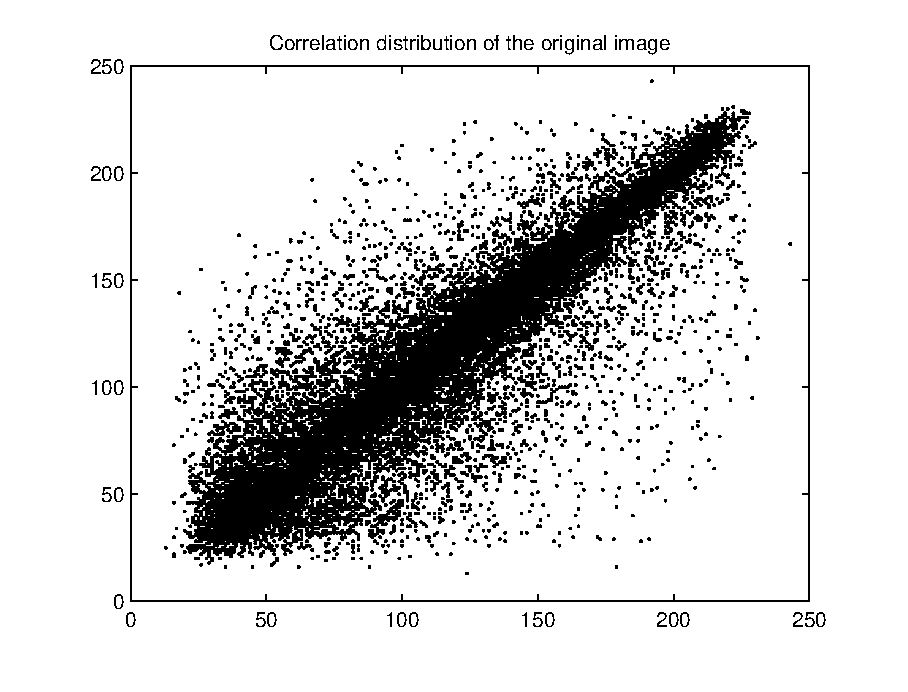
\includegraphics[scale = 0.35]{cd_lena.eps} %[Histogram of digitized laser]
}

\caption{(a) The original image. (b) The hidden image. (c) Correlation distribution of the original image. (d) Histogram of the original image.}
\label{Original}
\end{figure*}

Suppose that the size of the image is $M \times N$. The steps of the proposed information hiding
algorithm using the CIPRNG family (versions 1-3) are summed up below. Researches presented in this chapter have been formerly submitted/accepted/published in \cite{bfg12b:ip}.
\begin{enumerate}
\item Generate a pseudorandom sequence $S$ of length $M \times N$  using each CIPRNG method respectively.
\item Transform the image into a $M \times N$ integer sequence.
\item The LSBs (Least Significant Bits) of the image integer sequence are replaced by the generated random bits $S$. These random LSBs will be treated as a keystream.
\item The information (text or picture) to hide is transformed into a binary sequence.
\item The binary message is hiding into the random LSBs of the image sequence, by using the bitwise exclusive or operation between the two sequences, starting from a selected position acting as part of the secret key.
\end{enumerate}

As mentioned previously, pseudorandom sequences generated by the three CI methods, with two XORshift generators and a given image, are used in this application to process to an evaluation of the scheme.

\subsection{First Experimental Evaluation of the Proposed Scheme}

\subsubsection{The context}

The original image of size $713 \times 713$,
probably the most widely used test image for all kind of processing algorithms (such as compression and encryption),
 is depicted in Fig.~\ref{Original}-a.
Fig.~\ref{Original}-c presents its histogram, and Fig.~\ref{Original}-d shows the correlation distribution of two horizontal adjacent pixels in this original image.
Finally, information that must be hidden into it is the picture of Fig.~\ref{Original}-b, which has $89 \times 89$ pixels.

\begin{figure*}
\centering
\subfigure[]{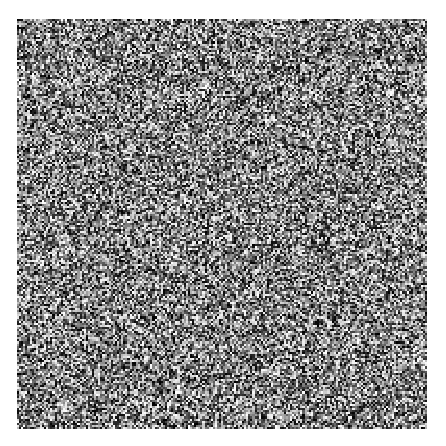
\includegraphics[scale = 0.55]{xor_ci_new.eps} %[Histogram of digitized laser]
}
\subfigure[]{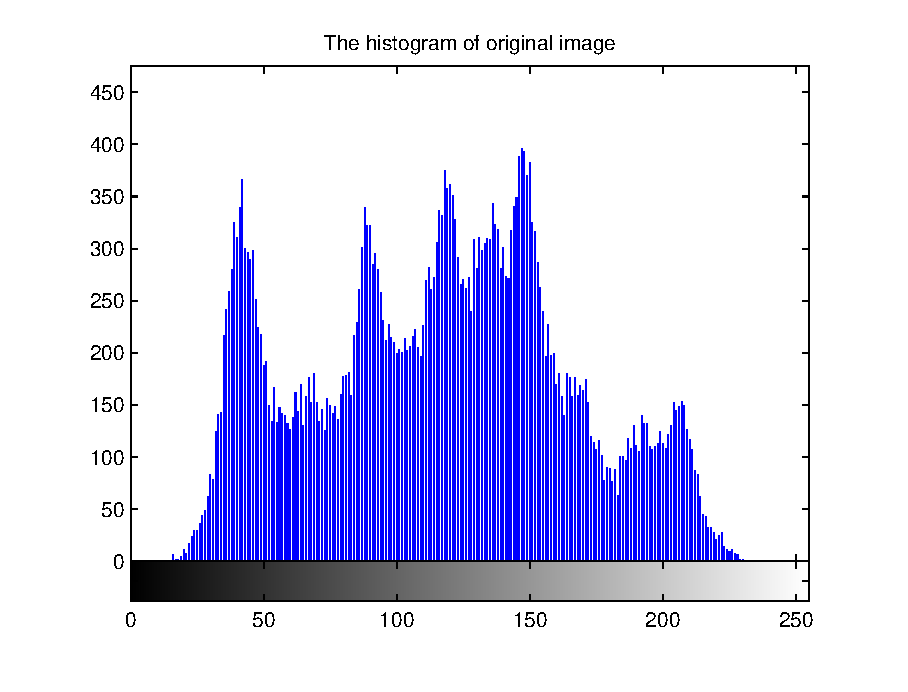
\includegraphics[scale = 0.35]{hist_xor_ci.eps} %[Histogram of digitized laser]
}
\subfigure[]{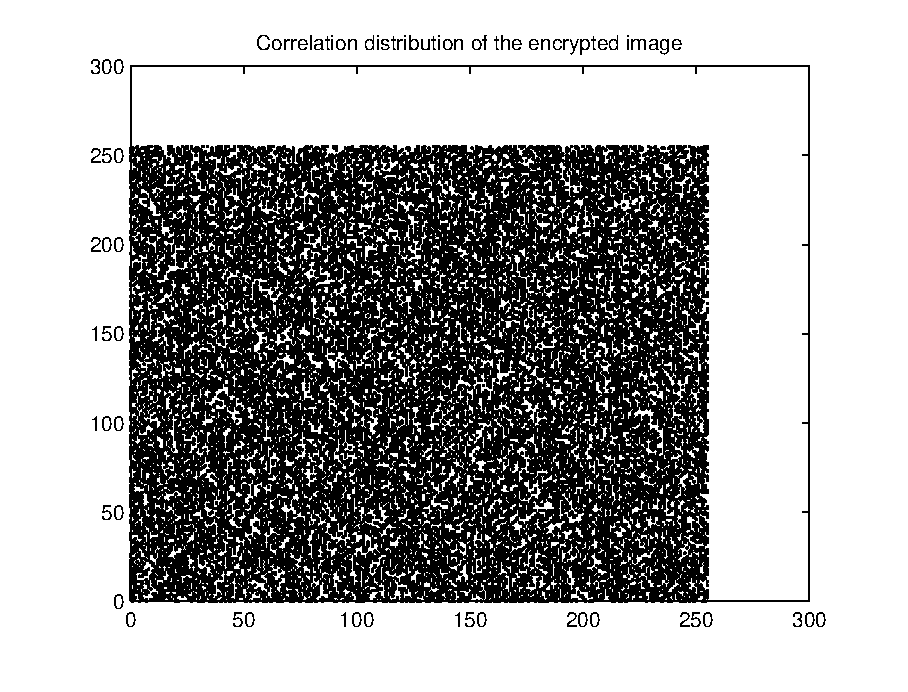
\includegraphics[scale = 0.35]{cd_xor_ci.eps} %[Histogram of digitized laser]
}
\caption{(a) The encrypted Lena (one-time pad using Version 3 CI). (b) Histogram of Fig.(a). (c) Correlation distribution of two adjacent pixels in Fig.(a)}
\label{Xor_CI}
\end{figure*}


\begin{figure*}
\centering
\subfigure[]{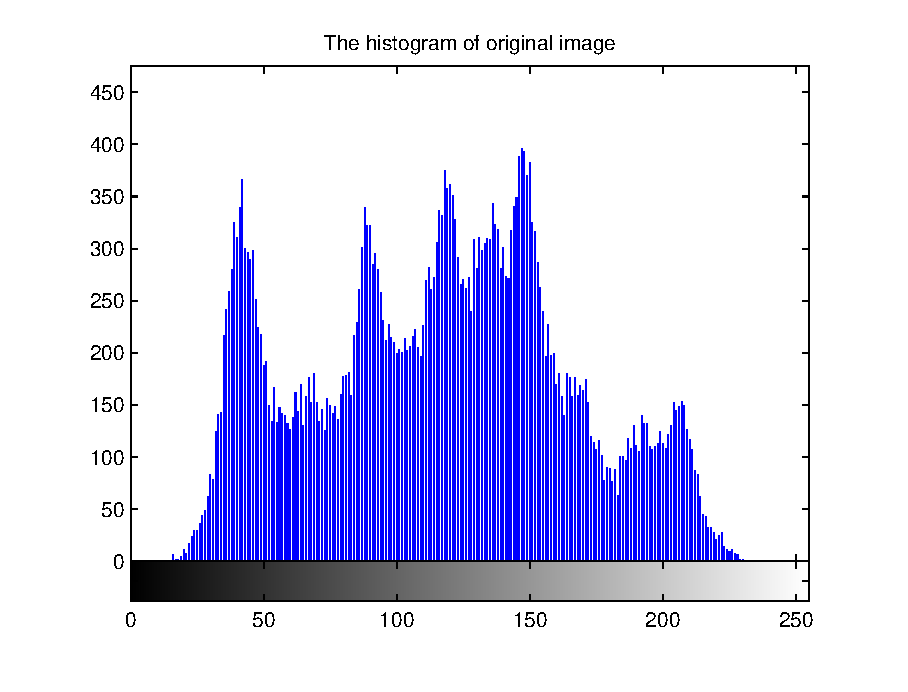
\includegraphics[scale = 0.29]{hist_xor_ci.eps} %[Histogram of digitized laser]
}
\subfigure[]{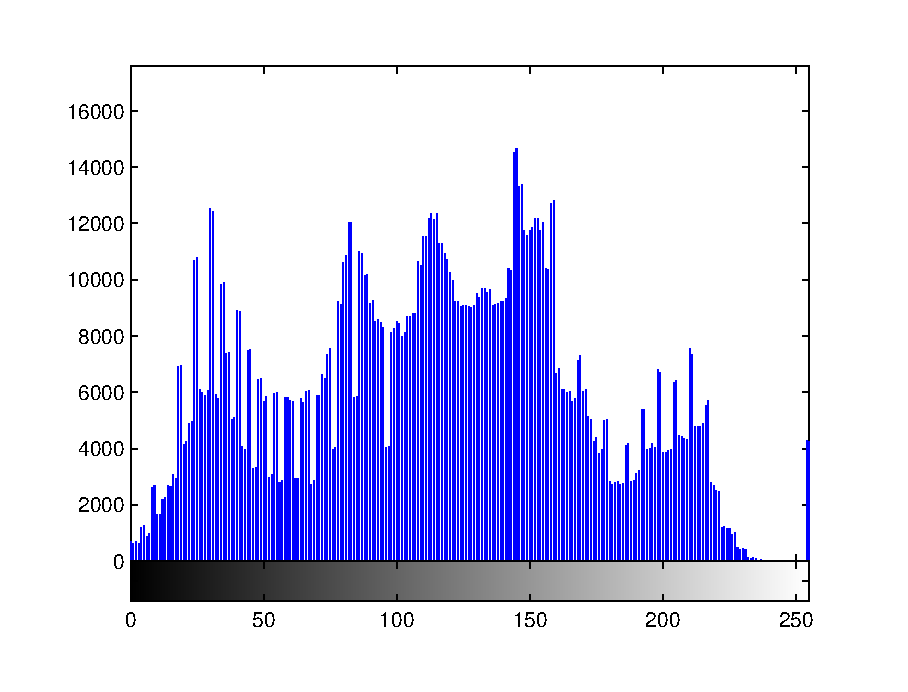
\includegraphics[scale = 0.29]{hist_xor_ci_info.eps} %[Histogram of digitized laser]
}
\subfigure[]{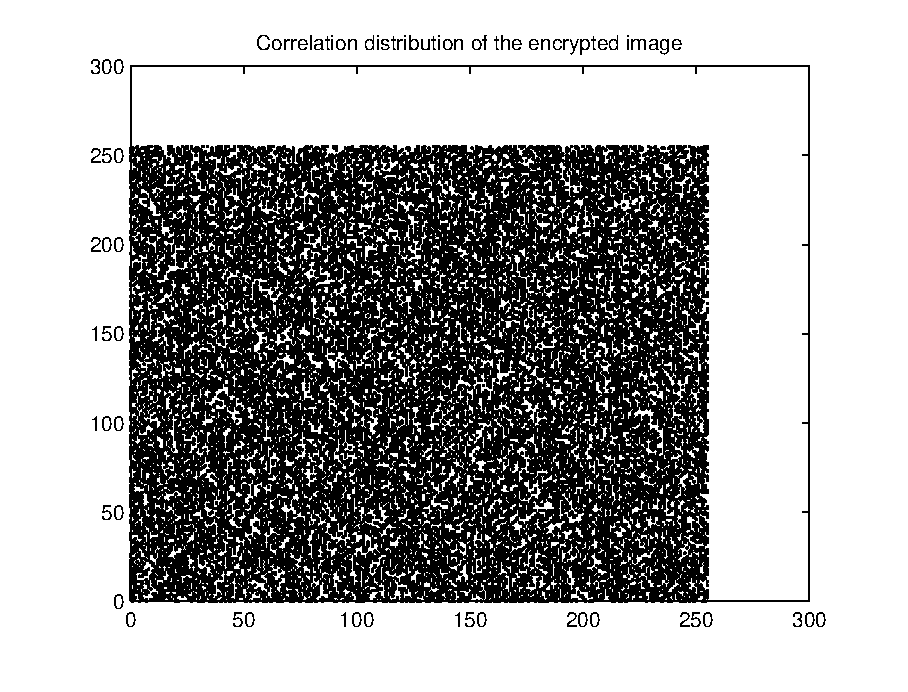
\includegraphics[scale = 0.29]{cd_xor_ci.eps} %[Histogram of digitized laser]
}
\subfigure[]{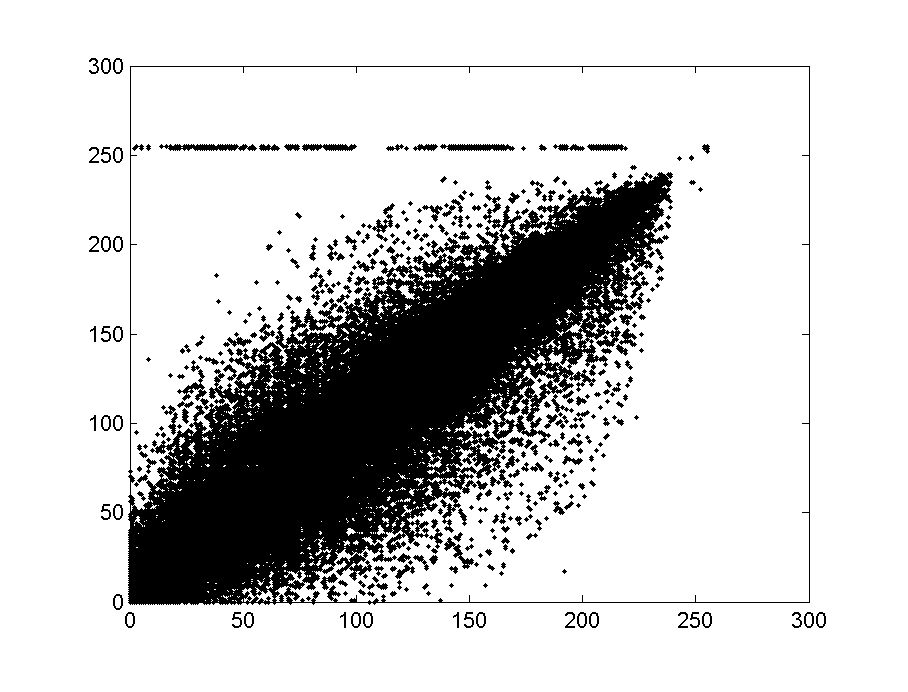
\includegraphics[scale = 0.29]{cd_xor_ci_info.eps} %[Histogram of digitized laser]
}
%\caption{ (a) Histogram of the random LSBs image using Version 3 CI. (b) Histogram of the random LSBs image using Version 3 CI with information hiding. (c) Correlation distribution of the random LSBs image using Version 3 CI. (d) Correlation distribution of the random LSBs image using Version 3 CI with information hiding.  }
\caption{ (a) Histogram of pixel values when LSBs are replaced by Version 3 CI. (b) Histogram of pixel values when LBSs are a hidden message xored with Version 3 CI. (c) Correlation distribution of two adjacent pixels in Fig.(a). (d) Correlation distribution of two adjacent pixels in Fig.(b).  }

\label{Xor_CI_hiding}
\end{figure*}


\subsubsection{Histogram and Horizontal Correlation}

Two XORshift generators are used to generate a random sequence based on the Version 1 CI method. Results are shown in Fig.~\ref{Old_CI_hiding}. Histograms and correlation distributions (Fig.~\ref{Old_CI_hiding}-a,b,c,d) are very closed to each other, leading to the
assumption that such a method can well protect the hidden information when facing statistical attacks.
The same experimental validation has been applied to the Version 2 CI method using two XORshift generators.
Such experiments lead to results that are shown in Fig.~\ref{New_CI_hiding}. These first results are
encouraging and confirm that simple histogram
and correlation evaluations cannot detect the
presence of hidden messages.
The same conclusion can be claimed when using the Version 3 CI generator, as it is depicted in Fig.~\ref{Xor_CI_hiding}.

%\subsubsection{Encryption with Version 3 CI}


\begin{figure*}
\centering
\subfigure[]{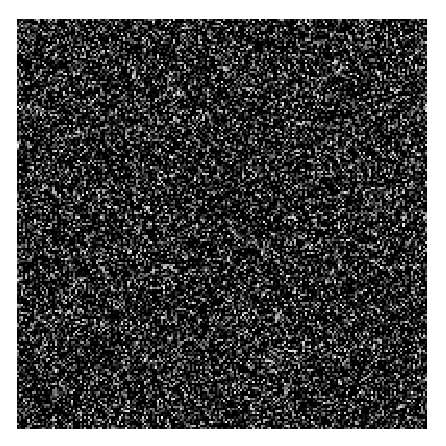
\includegraphics[scale = 0.15]{diff_old_ci.eps} %[Histogram of digitized laser]
}
\subfigure[]{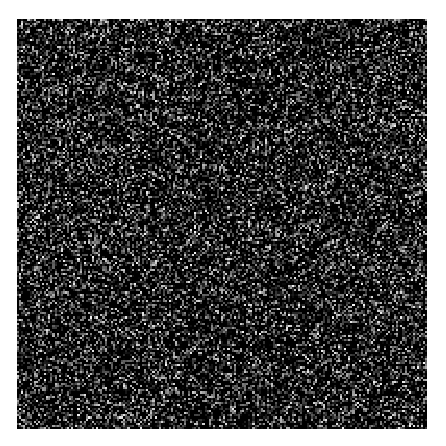
\includegraphics[scale = 0.15]{diff_new_ci.eps} %[Histogram of digitized laser]
}
\subfigure[]{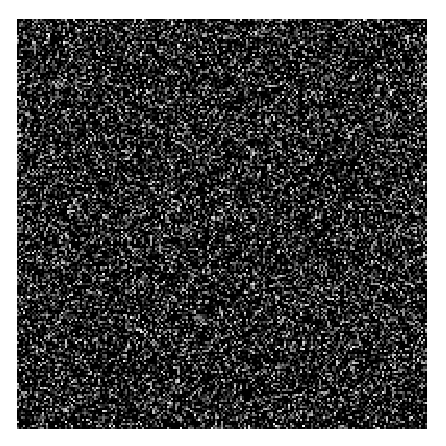
\includegraphics[scale = 0.15]{diff_xor_ci.eps} %[Histogram of digitized laser]
}
\caption{(a) The difference of two random LSBs image using Version 1 CI PRNG with slight change in initial condition. (b) The difference of two random LSBs image using Version 2 CI PRNG with slight change in initial condition (c) The difference of two random LSBs image using Version 3 CI PRNG with slight change in initial condition}
\label{diff}
\end{figure*}


\begin{table*}
\centering
\renewcommand{\arraystretch}{1.3}
\caption{Correlation coefficients of two adjacent pixels in all directions in the original image, random LSBs images and infomation intergraded random LSBs images}
\label{coefficients}
\centering
  \begin{tabular}{|l||c|c|c|}
    \hline
\backslashbox{\textbf{Image}} {\textbf{Direction}} & Horizontal & Vertical & Diagonal \\ \hline
 Original image& 0.9793& 0.9686& 0.9488 \\ \hline
 Version 1 CI  \\\hline
 no info &0.9792& 0.9686& 0.9488 \\ \hline
 intergrading info& 0.9792& 0.9686& 0.9488 \\ \hline
 Version 2 CI  \\\hline
 no info & 0.9793& 0.9686& 0.9488 \\ \hline
 intergrading info & 0.9793& 0.9686& 0.9488  \\ \hline
 Version 3 CI \\ \hline
 no info& 0.9793& 0.9686& 0.9487 \\ \hline
 intergrading info& 0.9793& 0.9686& 0.9487 \\ \hline
\end{tabular}
\end{table*}

\subsubsection{All directions correlation coefficients analysis}

Using an identical experimental evaluation than in~\cite{Chen2004749}, the correlation coefficients of the horizontal, vertical, and diagonal directions of all the concerned images (original, with random as LSBs, and with secret information in these LSBs) are shown in Table~\ref{coefficients}.
It can be experimentally deduced that the correlation properties of these images are very similar to each other.
So an attacker, whose intention is to analyze
these coefficients in order to detect possible
information hiding, cannot attain his/her goal
by such a simple experiment.

\subsubsection{Initial condition sensitivity}

One of the most important properties of the chaotic sequences is that they are very sensitive to their initial conditions.
This property can help to face an attacker who
has access to the whole algorithm and to an
approximation of the secret key.
His/her intention, in this attack scenario, is
to find the exact secret key (the seed of the
keystream and the position of the message), by
making small changes on this key.
If the keystream and the position do not change
a lot when the key is slightly updated, then the
attacker can converge by small changes to the used secret key.
In the experiments of Figure~\ref{diff}, we slightly alter the keys and try to extract the hidden information from the image.
We can conclude that such optimistic attempts
always fail in recovering the message.



\subsection{A small evaluation of Encryption}

The dissimulation has been obtained in this paper by using the CIPRNGs recalled previously as stream
cyphers:  encryption is the result of the use of the bitwise exclusive or (XOR) between the given message and pseudorandom sequences generated from various CIPRNGs. We can wonder whether an attacker, who has access
to the histogram of LSBs, can infer what kind of CIPRNG has been used as keystream.
For obvious reasons, these histograms should at least be uniform for each PRNG.

For illustration purpose, Lena has been encrypted by such method using each of the three kind of
CIPRNGs, and histogram and correlation distribution of the encrypted image have been computed. The resulting images are depicted in Fig.~\ref{Old_CI}
when using the Version 1 CI method, in Fig.~\ref{New_CI} for the Version 2 CI one, and in Fig.~\ref{Xor_CI} for the last PRNG recalled here.
We can show that this first reasonable requirement seems to be respected, even if this illustration
is not a proof.

\section{Conclusion}

We have %summarized in this chapter our previous contributions in the field of pseudorandom
%generators, and we have 
proposed, in this short application chapter, simple illustrative examples of use for information hiding.
The three first versions of the CIPRNGs family have been used here. 
%recalled here are namely the Version 1 CI, the Version 2 CI, and the Version 3 CI PRNGs.
For each generator,
firsts experimental evaluations of a simple information hiding scheme have been realized,
to illustrate that that an attacker using simple
statistics cannot determine easily, only by regarding the form of histograms or
 correlation distributions, the presence of an hidden message into a given document.
No evidence of dissimulation appears at first glance, when comparing histograms, correlation distribution, or all directions' correlation coefficients. Furthermore, experiments have illustrated high sensitivity to the secret parameters.
These simple evaluations do not imply the security of the proposed scheme, they only illustrate that the
use of the CIPRNGs for information hiding can be further investigated by more stringent tools
as steganalyzers and
mathematical proofs.
